%Atwood Machine
\newexp


\begin{tabbing}
\bf{Apparatus List:} \hspace{12pt} \=  Pasco ``smart pulley" \\
	\> Pasco DataStudio software \\
	\> Pasco 750 interface box \\
	\> bench clamp, right angle clamp, large supporting rod \\
	\> assorted weights \\
	\> digital balance (accurate to 0.1 gram) \\
	\> foam ``landing pad" for weights \\
\end{tabbing}

\section*{Before Lab}

It is straightforward to show, using Newton's laws, that the
acceleration $a$ of the system of masses shown Fig.~\ref{fig:atwood}
below is given by
\[
 a = {{M - m} \over {M + m}}\; g
\]
where $g$ is the
acceleration of gravity and $M$ and $m$ the two masses.
In your lab notebook, you should make a
careful force diagram for each mass and derive this result.
See your textbook or your instructor if you need help.  We will want
to compare the predictions of this theoretical
equation to the experimental acceleration we measure directly.


\section*{Introduction}

\begin{figure}[!hbt]     %Atwood machine diagram, atwood.eps
\begin{center}
{\resizebox{2in}{!}{{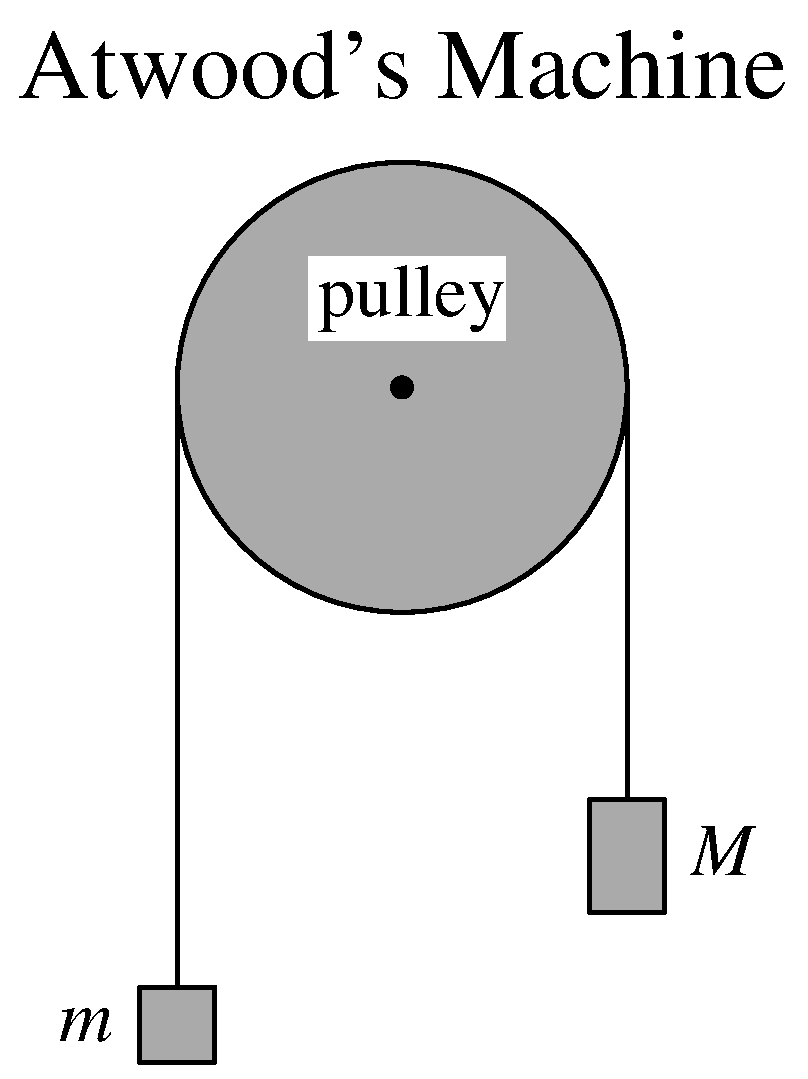
\includegraphics{atwood2.eps}}}}
\end{center}
%\vspace{3in}
%\special{eps:atwood.eps}
\caption{Diagram of Atwood Machine.
          \label{fig:atwood}}
\end{figure}
In 1784 Rev.\ George Atwood devised a laboratory apparatus 
to verify the Newton's laws of uniformly accelerated motion.
An Atwood machine (shown Fig.~\ref{fig:atwood}) uses weights and pulleys to 
reduce the free-fall acceleration so it can be more easily measured.
In this experiment we will use
the computer to record the
velocity of the masses as a function of time.  From these data, we can
calculate the actual acceleration and compare to the theoretical result
you derived for the pre-lab.

Increasingly, scientists and engineers use computers to acquire data
automatically from experiments.  In this experiment, we will introduce
a hardware and software system designed by Pasco Scientific, which
allows us to 
%connect interface hardware through an SCSI port, and 
record data from a wide
range of apparatus automatically, using the Pasco DataStudio
software for Windoze.  We will use this same system in
other experiments in this course.



\section*{Apparatus and Procedure}

Please note first of all that the Pasco ``smart pulley" is fragile.
Be careful in working with it!  {\bf In particular, be sure that you
choose
a length of string such that it is impossible for the upward-moving
weight to strike the pulley!}

First notice how the pulley works.  There is a beam of light that
passes from one side of the pulley to the other.  As the pulley turns,
this light beam is interrupted by one of the pulley spokes (a ``photogate"), and a
signal is transmitted to the computer.  The system measures
directly the time from one interruption of the light beam to the next.
Since the pulley has ten spokes, we are measuring the time it takes
for the pulley to move through an angle of $36^{\circ}$ --- 1/10 of a
circle. If
we know the radius of the pulley, it is not hard to calculate how fast
the string is moving as the pulley turns.
We will be talking about how to do this calculation later in the
semester; but see if you can figure it out now.

{\bf NOTE:} The Pasco software uses a built-in ``calibration constant"
to convert these times into linear velocities.  Unfortunately, this
calibration constant is given to only two significant figures.  As a
result you should expect that the Pasco velocities are systematically
a few percent high or low.  In this course we rarely encounter important
systematic errors; instead we've concentrated on ``random errors": measurement
deviations which vary in  sign and magnitude when the measurements are repeated.
Unlike random errors, systematic errors do not signal their presence
on re-measurement.  As a result systematic errors are difficult to detect;
they are almost always behind apparent discrepancies in published measurements.
Experimenters usually minimize random errors by averaging over  larger datasets
(see below: the standard deviation of the mean $\propto 1/\sqrt{N}$), however
for sufficiently large $N$ the silent systematic errors will dominate the
visible random errors.  Beware!


% uncertainty in the velocities.
%(remember our discussion from the Reaction Time experiment about the
%difference between systematic and random uncertainties).

After your lab instructor shows you how the apparatus works, take some
time to become familiar with it.  See how the string fits over the
pulley, hang some masses from each end, and do a few test runs.  It
is probably best to keep accelerations reasonably small.  Here
are a few guidelines:
\begin{itemize}
\item Mount the pulley as high on the vertical rod as you easily can.
Be
sure the rod is stable, and does not tend to shake or vibrate easily.
%
\item Do not hang a total of more than 600 grams from the pulley
(both sides).
%
\item Note that the larger the total mass, and the smaller the
difference
between the two masses, the smaller the acceleration should be.
%
\item {\bf Be absolutely sure, before you do any test runs, that your
string
is long enough that the upward-moving mass cannot strike the pulley! }
\end{itemize}

\section*{Taking the Data}

Here are some guidelines for taking a set of velocity vs.\ time data,
from which you can calculate the acceleration.
Use these guidelines to develop your own procedure, and {\bf record}
that procedure in comprehensive detail in your lab book, {\bf while}
(not after) you are taking the data.

We will take data for two separate sets of masses.  Try to choose
values for which the accelerations differ by at least a factor of two;
but keep both accelerations reasonably small.

For each set of masses, take four separate sets of data.  Thus, you
will have a total of 8 runs for this experiment.

Guidelines for taking data:
\begin{itemize}
\item Measure the masses carefully on the digital balance.  If you are
combining several objects to be $M$ (or $m$),
%using more than one mass for either $m$ or $M$, 
measure the masses
together---do not measure the individual masses and add them later.
Why?
%
\item Set up $m$ and $M$ on the string.  The lighter mass should be
as close to the floor as possible.
%
\item Develop a procedure for releasing the masses---be sure they do
not have a tendency to sway as they move.
%
\item One should person click the Start button on the Pasco screen, then the
other person releases the masses.
As soon as the descending mass
strikes the floor, click on the Stop button.  You should now have a
set of data for velocity vs.\ time.   Examine the data on the graph in
the Pasco DataStudio program, and be sure you understand how to
use it to find the acceleration of the masses.
%
\end{itemize}

\section*{Data Reduction and Analysis}
\subsection*{Using \WAPP to find the acceleration}

We will move the velocity vs.\ time data to \WAPP to find the acceleration.  To do so:
\begin{itemize}
\item Start up a web browser, and go to the \WAPP web site.  Select
no $x$ errors (uncertainty in time is negligible) and a formula
for $y$ error. The uncertainty in velocity produced by the smart pulley
seems to be about 0.003~m/sec (a constant).  Click on ``Do Bulk".
%
\item Go back to the Pasco program, and select only those velocity vs.
time data that you want to fit.  Note that as you select the data on
the graph, it is also selected in the table. %Select (click on) the table window.
%
\item Select ``Copy" from the Edit menu (or use control-C).
%
\item Now switch to the \WAPP bulk entry form and paste your data in.
In addition to the numbers, DataStudio will include text describing the data:
this text must be removed!
Select a linear functional form and Submit that data.
%
\item You will be taking eight sets of data.  
It is a good idea to save this data by pasting it into an Excel spreadsheet.
%
%\item Select your data on the spreadsheet, move it to the data screen,
%and do your least-squares fit to find the acceleration.
%\begin{itemize}
%\item For the uncertainty in velocity, use 0.003 m/sec.
%(This estimate is based on limited experience; let your instructor
%know if your reduced chi-squared value seems off.)
%
%\item Parameter estimates: Use your theoretical value of the
%acceleration for the slope; for the intercept, choose zero, since the
%initial speed of the masses will be small.
\end{itemize}
%
You do not need to print your fit report or plot; but do 
copy into your notebook and spreadsheet the resulting value for
the slope and its uncertainty (the parameter $B$).
%back to the
%spreadsheet, and from the Data menu, choose Data/Get Fit Results from
%Fit Screen.  This step will open a new worksheet.  It might be easiest
%to cut the slope and its uncertainty (the parameter $B$) and paste it
%into the same worksheet with your data.
%\end{itemize}

{\bf For each data set, you
should, at this point, have a value of acceleration, and the
uncertainty in the acceleration, from your least-squares fit.}
Group equivalent experimental situations in a column of
your spreadsheet; display in nearby cells the masses used and
theoretical prediction for the acceleration from Eq.~\ref{eq:atwood.a}.
%You might also want to record your two masses on this worksheet, and
%calculate the theoretical value of the acceleration.  
Put enough text
in the worksheet so readers can easily see what each number
represents.  Include units, of course!


\subsection*{Uncertainty in the experimental value of the acceleration}
The uncertainty in each acceleration, which you obtain from your
least-squares fit, applies to that particular run.  But are there
variations from one run to the next, as was the case in the previous lab? We will investigate that
question in the following way:
\begin{itemize}
\item For each set of masses, collect the four values of the
acceleration that you found from your least-squares fits.
%
\item Calculate the average acceleration (spreadsheet function: {\tt average()}), the standard deviation
(spreadsheet function: {\tt stdev()}), and
the standard deviation of the mean ({\tt stdev()/sqrt(4)}) \label{atwood.sdev.mean} (see Appendix A, page~\pageref{sdev.mean}).
Remember to ``self-document" these spreadsheet calculations.
Note that the standard
deviation of the mean should represent the uncertainty in the
average acceleration.
If reproducibility is not a problem,
the standard deviation will be
comparable to the uncertainties from your least-squares fits.  %(Note
%that you can use a spreadsheet function to calculate the standard
%deviation---see the on-line help.)
% In addition, calculate the standard deviation of the mean.  What additional information does this quantity give you?
\end{itemize}

\subsection*{Uncertainty in the theoretical value of
the acceleration}

As noted above, the theoretical value of the acceleration is given by

\begin{equation}
 a = {{M - m} \over {M + m}}\; g \label{eq:atwood.a}
\end{equation}
We will want to compare this theoretical value with your experimental
values.  In order to do so, we must know the uncertainty in the
theoretical value based on the measured uncertainties in the masses
$M$ and $m$.  It turns out to be fairly difficult to calculate the
uncertainty in the acceleration $a$ using the error propagation techniques developed in
Appendix A,
so we will do it using the ``high-low" game described on page \pageref{par:high.low.game}. %``experimentally."  
Change each mass (up and also down) by the measured
uncertainty (0.1~gm, for the digital balance that we use) and see what
happens to the acceleration.  Half the difference between the largest
and smallest calculated values of acceleration is a rough estimate of
the uncertainty.

Include your theoretical accelerations (with uncertainty) in your
spreadsheet of experimental accelerations.  Print it out (but do not print
the the eight long columns of actual data).

\section*{Table of Results and Conclusion}

In most experiments, it is important to summarize all your
numerical results in your conclusions section.  For each set of
masses, make a table that includes
\begin{enumerate}
\renewcommand{\labelenumi}{(\alph{enumi})}
\item  the theoretical value of the acceleration, with uncertainty;
%
%\item your value of the acceleration for each of your four runs with
%that set of masses, with uncertainty (these values are the ones from
%the least-squares fits); and
%
\item the average value and standard deviation of the mean for the
four measurements.
\end{enumerate}
Of course, every number should be properly recorded (sigfigs, units, error).
You can make this table in your spreadsheet (but sometimes it is not worth
the struggle to get Excel to properly display sigfigs).
%; print out the table portion
%and supporting data/calculations (but not eight long columns of actual data)
%and tape it into your lab notebook.
%As always, put in enough text so the printout can be read easily by someone else.
%(Formating cells for the proper number of significant digits need only
%be done for the final table results; self-document every spreadsheet calculation.)

In your conclusion, you should discuss, separately for each set of
data, whether the theoretical and experimental values for the
acceleration agree, within the uncertainties of the experiment.  You
should also discuss whether the uncertainties in the least-squares
fits are consistent with the standard deviations (i.e., is reproducibility
a problem).
If theory and experiment do not agree, are there sources of systematic error that
might account for such an inconsistency?  (One is mentioned
above---the
calibration constant of the ``smart pulley;" what other systematic
errors might be present in this experiment?)

\section*{Quick Report Card}
Properly report (sigfigs, units, error) (a) and (b) above from your final table.


